\documentclass{beamer}

% --------------------------------------------------------------------
% THEME AND APPEARANCE
% --------------------------------------------------------------------
% Choose a theme for the presentation.
% Popular themes: Madrid, Berlin, Boadilla, CambridgeUS, Copenhagen,
% Darmstadt, Dresden, Frankfurt, Goettingen, Hannover, Ilmenau,
% Juanlespins, Luebeck, Malmoe, Marburg, Montpellier, PaloAlto,
% Pittsburgh, Rochester, Singapore, Szeged, Warsaw.
\usetheme{CambridgeUS}


% Choose a color theme.
% Popular color themes: beaver, beetle, crane, dolphin, dove, fly,
% lily, orchid, rose, seagull, seahorse, whale, wolverine.
\usecolortheme{default}
% add a logo to the title page (optional)
%\titlegraphic{\includegraphics[height=1.5cm]{logo.png}}

% --------------------------------------------------------------------
% PACKAGES
% --------------------------------------------------------------------
\usepackage{tikz}     % For drawing diagrams
\usetikzlibrary{positioning, arrows.meta}
\usepackage{graphicx} % For including images
\usepackage{booktabs} % For professional quality tables
\usepackage{minted}   % For syntax-highlighted code blocks.
                      % This requires the 'pygments' Python package to be installed.
                      % You may need to compile with the -shell-escape flag (e.g., pdflatex -shell-escape main.tex)
\usepackage{hyperref}

% --------------------------------------------------------------------
% PRESENTATION METADATA
% --------------------------------------------------------------------
\title[Some Fun With Bevy]{An Overview to Game Development Using Rust}
\subtitle{A Toxic Relationship With Rust}
\author{Marti}
\institute{OmniMeet}
\date{November 25, 2025}

\begin{document}

% --------------------------------------------------------------------
% TITLE PAGE
% --------------------------------------------------------------------
\begin{frame}
  \titlepage
\end{frame}

% --------------------------------------------------------------------
% TABLE OF CONTENTS
% --------------------------------------------------------------------
% Uncomment the following frame to show an outline at the beginning.
% \begin{frame}{Outline}
%   \tableofcontents
% \end{frame}

% --------------------------------------------------------------------
% SECTIONS AND FRAMES
% --------------------------------------------------------------------
\AtBeginSection[]
{
  \begin{frame}{Outline}
    \tableofcontents[currentsection,currentsubsection]
  \end{frame}
}

\section{What is Bevy?}
% make me a slide with bevy logo and some text about bevy
\begin{frame}{What is Bevy?}
  \frametitle{Bevy Game Engine}
  \begin{columns}[T] % T aligns columns at the top
    \begin{column}{0.4\textwidth}
      \includegraphics[width=\textwidth]{bevy_logo.png} % Placeholder for Bevy logo
    \end{column}
    \begin{column}{0.6\textwidth}
      \textbf{Bevy} is an open-source data-driven game engine built in Rust.
      \begin{itemize}
        \item It emphasizes simplicity, modularity, and performance.
        \item Bevy uses an Entity-Component-System (ECS) architecture.
        \item It provides a range of features including 2D/3D rendering, audio, input handling, and more.
      \end{itemize}
    \end{column}
  \end{columns}
\end{frame}
\section{Why use Bevy for game development?}
\begin{frame}{Why use Bevy for game development?}
  \frametitle{Advantages of Bevy}
  \begin{itemize}
    \item \textbf{Rust Language}: Memory safety without garbage collection, zero-cost abstractions, and fearless concurrency.
    \item \textbf{ECS Architecture}: Promotes clean code organization, scalability, and high performance through data-oriented design.
    \item \textbf{Cross-Platform}: Deploy to Windows, macOS, Linux, Web (WASM), iOS, and Android from a single codebase.
    \item \textbf{Open Source}: MIT/Apache 2.0 licensed, actively maintained by a vibrant community.
    \item \textbf{Code-Driven}: Pure code workflow with no lock-in to proprietary editors (Official editor \href{https://bevy.org/news/bevys-fifth-birthday/\#bevy-editor-design}{in development}).
    \item \textbf{Modular Design}: Use only what you need - built as a collection of plugins you can mix and match.
  \end{itemize}
\end{frame}
\begin{frame}{Why not use Godot or Unity?}
  \frametitle{Bevy vs Other Engines}
  \begin{itemize}
    \item \textbf{Lightweight}: Lightweight compared to larger engines.
    \item \textbf{Flexibility}: More control over low-level systems and architecture.
    \item \textbf{Paradigm}: ECS is still not really popular in general.
  \end{itemize}
\end{frame}
\section{How does Bevy works?}
\subsection{ECS Architecture}

\begin{frame}{ECS Architecture}
  \frametitle{Entity-Component-System (ECS)}
  
  \begin{center}
    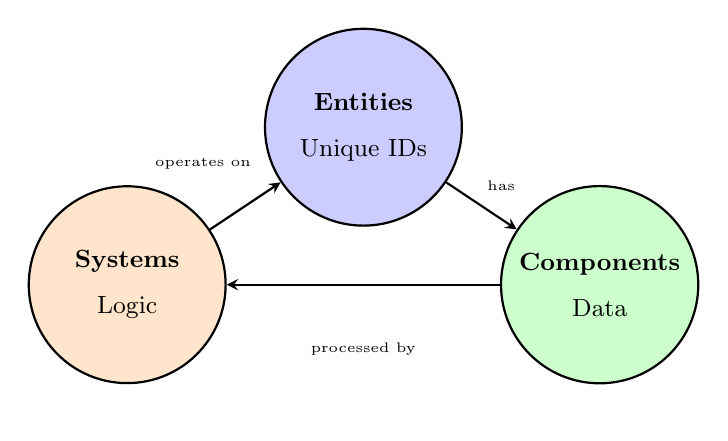
\begin{tikzpicture}[
      node distance=3.5cm,
      every node/.style={draw, circle, minimum size=2.5cm, align=center, font=\small, thick},
      arrow/.style={->, >=stealth, thick}
    ]
      \node[fill=blue!20] (entity) at (0,2) {\textbf{Entities}\\[0.2cm]Unique IDs};
      \node[fill=green!20] (component) at (3,0) {\textbf{Components}\\[0.2cm]Data};
      \node[fill=orange!20] (system) at (-3,0) {\textbf{Systems}\\[0.2cm]Logic};
      
      \draw[arrow] (entity) -- (component) node[midway, above right, draw=none, minimum size=0] {\tiny has};
      \draw[arrow] (component) -- (system) node[midway, below, draw=none, minimum size=0] {\tiny processed by};
      \draw[arrow] (system) -- (entity) node[midway, above left, draw=none, minimum size=0] {\tiny operates on};
    \end{tikzpicture}
  \end{center}
    
  \vspace{-0.6cm}
  \begin{columns}[T]
    \begin{column}{0.3\textwidth}
      \centering
      \colorbox{blue!20}{\parbox{0.9\textwidth}{
        \centering
        \textbf{\large Entities}\\[0.3cm]
        \small Unique identifiers representing objects in the game world
      }}
    \end{column}
    \begin{column}{0.3\textwidth}
      \centering
      \colorbox{green!20}{\parbox{0.9\textwidth}{
        \centering
        \textbf{\large Components}\\[0.3cm]
        \small Data containers that hold attributes of entities
      }}
    \end{column}
    \begin{column}{0.3\textwidth}
      \centering
      \colorbox{orange!20}{\parbox{0.9\textwidth}{
        \centering
        \textbf{\large Systems}\\[0.3cm]
        \small Logic that operates on entities with specific components
      }}
    \end{column}
  \end{columns}
\end{frame}

\begin{frame}
  \includegraphics[width=0.5\textwidth]{cow.png} % Placeholder for an image illustrating ECS  
\end{frame}



\begin{frame}
  \frametitle{Traditional OOP Approach}
  \framesubtitle{Shitty Inheritance Hierarchy}
  
  \begin{columns}[c]
    \begin{column}{0.4\textwidth}
      \centering
      \includegraphics[width=0.9\textwidth]{cow.png}
    \end{column}

    \begin{column}{0.8\textwidth}
      
      \resizebox{7cm}{!}{

      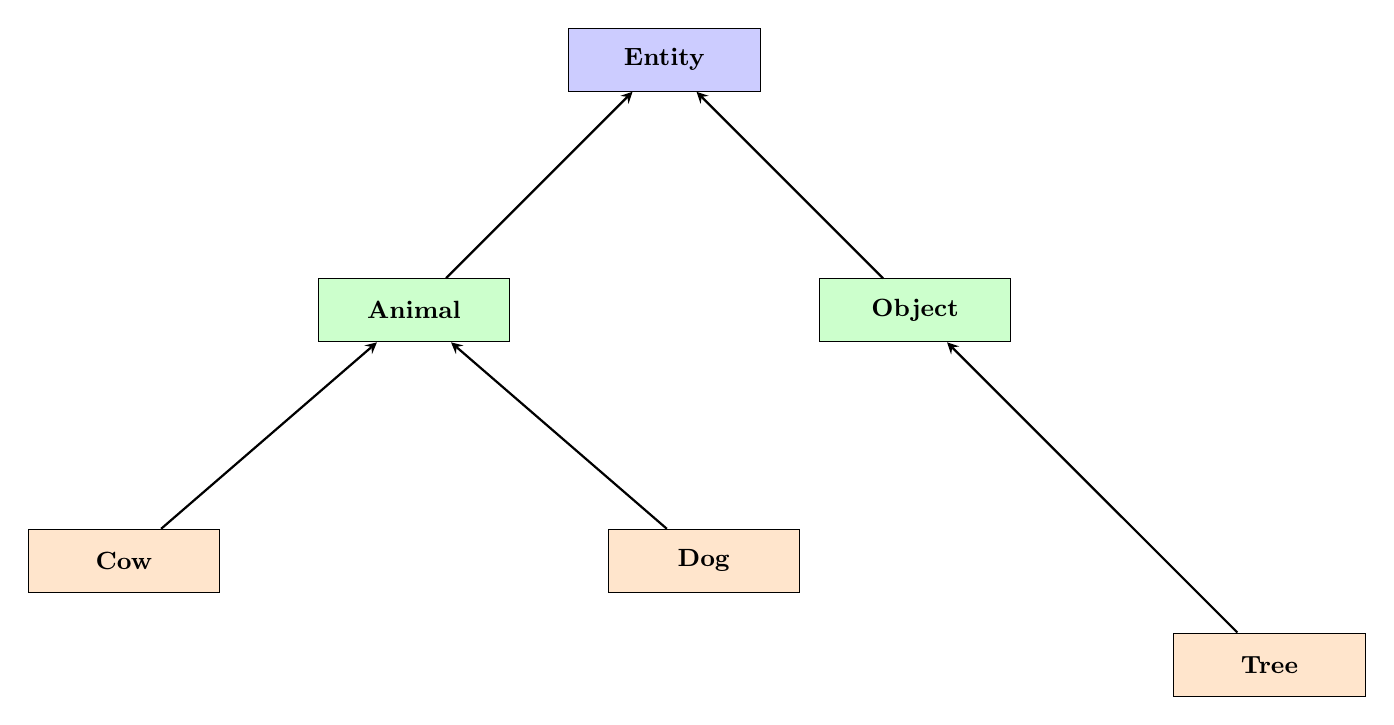
\begin{tikzpicture}[
        node distance=4.5cm and 2cm,
        class/.style={rectangle, draw, fill=blue!10, text width=2.2cm, align=center, minimum height=0.8cm, font=\small},
        arrow/.style={->, >=stealth, thick}
      ]
        % Top level
        \node[class, fill=blue!20] (entity) {\textbf{Entity}};
        
        % Second level
        \node[class, fill=green!20, below left of=entity] (animal) {\textbf{Animal}};
        \node[class, fill=green!20, below right of=entity] (object) {\textbf{Object}};
        
        % Third level - under Animal
        \node[class, fill=orange!20, below left of=animal, xshift=-0.5cm] (cow) {\textbf{Cow}};
        \node[class, fill=orange!20, below right of=animal, xshift=0.5cm] (dog) {\textbf{Dog}};
        
        % Third level - under Object
        \node[class, fill=orange!20, right of=dog, below of=object ] (tree) {\textbf{Tree}};
        
        % Arrows
        \draw[arrow] (animal) -- (entity);
        \draw[arrow] (object) -- (entity);
        \draw[arrow] (cow) -- (animal);
        \draw[arrow] (dog) -- (animal);
        \draw[arrow] (tree) -- (object);
      \end{tikzpicture}
      }
    \end{column}
  \end{columns}
      
  %\vspace{0.3cm}
  %\centering
  %\small \textit{Traditional class inheritance creates rigid hierarchies}
\end{frame}









% poo
\begin{frame}
  \begin{columns}[c]

    
    \begin{column}{0.3\textwidth}
      \centering
      \includegraphics[width=1\textwidth]{cow.png}
    \end{column}

    \begin{column}{0.8\textwidth}
      \centering
      \resizebox{3cm}{!}{
      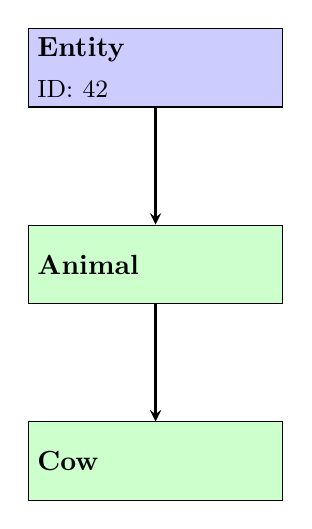
\begin{tikzpicture}[
        node distance=2.5cm,
        class/.style={rectangle, draw, fill=blue!10, text width=3cm, align=left, minimum height=1cm},
        arrow/.style={->, >=stealth, thick}
      ]
        % Entity
        \node[class, fill=blue!20] (entity) {\textbf{Entity}\\[0.1cm]\small ID: 42};
        
        % Components
        \node[class, fill=green!20, below of=entity] (animal) {\textbf{Animal}\\[0.1cm]\small};
        \node[class, fill=green!20, below of=animal] (cow) {\textbf{Cow}\\[0.1cm]\small};
                
        % Arrows
        \draw[arrow] (entity) -- (animal) node[midway, right, draw=none]{};
        \draw[arrow] (animal) -- (cow) node[midway, right, draw=none]{};
        
      \end{tikzpicture}
      }
    \end{column}
  \end{columns}
\end{frame}
% end poo



\begin{frame}
  \frametitle{ECS Architecture}
  \framesubtitle{Example: A Cow Entity}
  
  \begin{columns}[c]
    \begin{column}{0.55\textwidth}
      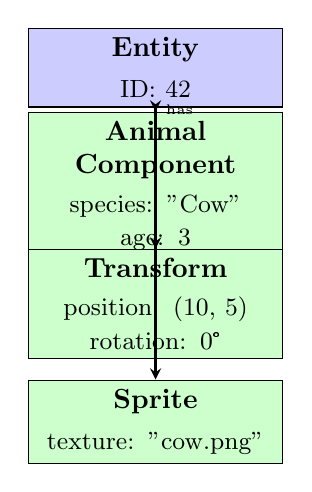
\begin{tikzpicture}[
        node distance=1.5cm,
        class/.style={rectangle, draw, fill=blue!10, text width=3cm, align=center, minimum height=1cm},
        arrow/.style={->, >=stealth, thick}
      ]
        % Entity
        \node[class, fill=blue!20] (entity) {\textbf{Entity}\\[0.1cm]\small ID: 42};
        
        % Components
        \node[class, fill=green!20, below of=entity] (animal) {\textbf{Animal Component}\\[0.1cm]\small species: "Cow"\\age: 3};
        
        \node[class, fill=green!20, below of=animal] (transform) {\textbf{Transform}\\[0.1cm]\small position: (10, 5)\\rotation: 0°};
        
        \node[class, fill=green!20, below of=transform] (sprite) {\textbf{Sprite}\\[0.1cm]\small texture: "cow.png"};
        
        % Arrows
        \draw[arrow] (entity) -- (animal) node[midway, right, draw=none] {\tiny has};
        \draw[arrow] (entity) -- (transform);
        \draw[arrow] (entity) -- (sprite);
      \end{tikzpicture}
    \end{column}
    
    \begin{column}{0.4\textwidth}
      \centering
      \includegraphics[width=0.8\textwidth]{cow.png}
      
      \vspace{0.5cm}
      \small \textit{A cow entity is composed of multiple components that define its data}
    \end{column}
  \end{columns}
\end{frame}



\subsection{Bevy's Rendering Pipeline}
\begin{frame}{Bevy's Rendering Pipeline}
  \frametitle{Rendering in Bevy}
  \begin{itemize}
    \item Bevy uses a modern rendering pipeline based on wgpu.
    \item Supports both 2D and 3D graphics.
    \item Provides built-in shaders and materials.
  \end{itemize}
\end{frame}


\section{Building a simple game with Bevy.}



\begin{frame}{Introduction Slide}
  \frametitle{What is this presentation about?}
  So lets beging with an overview for what we can expect from this presentation.
  
  \begin{itemize}
    \item What is Bevy?
    \item Why use Bevy for game development?
    \item How does bevy works?
    \item Building a simple game with Bevy.
  \end{itemize}
\end{frame}


\section{Bevy Basics}


\section{Core Content}

\begin{frame}{A Slide with Columns}
  \frametitle{Two-Column Layout}
  
  \begin{columns}[T] % T aligns columns at the top
    \begin{column}{0.5\textwidth}
      \textbf{Left Column}
      \begin{itemize} 

        \item Perfect for placing text next to an image or a chart.
        \item This column takes up 50% of the text width.
      \end{itemize}
    \end{column}
    \begin{column}{0.5\textwidth}
      \textbf{Right Column}
      %\p{\includegraphics[width=\textwidth]{placeholder.png}} % Placeholder for an image
      \centering \footnotesize{Remember to add an image named 'placeholder.png' in your project directory.}
    \end{column}
  \end{columns}
\end{frame}

\begin{frame}[fragile]{Code Example}
  \frametitle{Showing Off Some Code}
  % The 'fragile' option is needed for frames with verbatim content like code.
  \begin{minted}{rust}
fn main() {
    println!("Hello, Beamer!");
}
  \end{minted}
\end{frame}

\section{Conclusion}

\begin{frame}{Conclusion}
  \frametitle{Thank You!}
  
  \begin{center}
    \Huge Questions?
  \end{center}
\end{frame}

\end{document}